\documentclass[10pt, a4paper] {article}
\usepackage[utf8]{inputenc}
\usepackage [polish]{babel}
\usepackage[T1]{fontenc}
\usepackage{graphicx}
\usepackage{caption}
\usepackage{float}

\graphicspath{{images/}}

\title {\textbf{Wypożyczalnia pojazdów} \\
Projekt grupowy}
\author {Michał Brus, Łukasz Tumialis, Rafał Bednarz}
\date {\today}

\begin{document}

\maketitle

\section {Opis}
Program symuluje wypożyczalnię samochodów.
\section{Klasy i metody}
Program składa się z następujących klas:
\begin {enumerate}
	\item VehicleRental - główna klasa
	\item Customer - klasa klienta
	\item Vehicle - klasa pojazd:
	\begin {itemize}
		\item Car - klasa pochodna samochód
		\item Truck - klasa pochodna ciężarówka
	\end{itemize}
	\item MyStack - klasa stosu
\end {enumerate} 


Klasy Vehicle, Customer i VehicleRental są ze sobą zaprzyjaźnione.

\subsection {VehicleRental}
Klasa VehicleRental składa się z 3 wektorów:
\begin{itemize}
	\item CustomerList
	\item CarList
	\item TruckList
\end{itemize}
 i stosu, na którym zapisujemy historię operacji. \\
 
 
\textbf{Metody klasy VehicleRental:}
\begin{itemize}
	\item Menu - metoda odpowiadająca za interaktywne menu
	\item ShowOperationsHistory - wyświetla historię operacji na obiektach
	\item Rent - odpowada za proces wypożyczenia pojazdu
	\item Payment - proces opłaty
	\item Return - zwrot pojazdu do wypożyczalni
	\item ShowVehicleList, ShowCustomerList - wyświetlanie listy pojazdów/klientów
	\item ShowInfo - funkcja zaprzyjaźniona, która wyświetla szczegółowe informacje o danym obiekcie
\end{itemize}

\subsection{Customer}
Klasa posiada typowe informacje jak:
\begin {itemize}
	\item Imię i nazwisko
	\item PESEL
	\item Typ prawa jazdy
	\item Czy aktualnie wypożycza?
	\item Obciążenie konta
\end{itemize}


oraz odpowiedniki metod VehicleRental.
\subsection{Vehicle}
Klasa posiada informacje ogólne o pojeździe:
\begin{itemize}
	\item Numer rejestracyjny
	\item Nazwa
	\item Rok produkcji
	\item Stan
	\item Czy można wypożyczyć?
	\item Czy pojazd jest sprawny?
\end{itemize}


Dodatkowo klasy Car i Truck posiadają dodatkowo odpwoiednio \textit{Ilość siedzeń} i \textit{Pojemność}.

\subsection{MyStack}
Klasa oparta na \textit{template}, w naszym przypadku odpowiada za przechowywanie historii operacji na obiektach. \\


Metody klasy MyStack:
\begin{itemize}
	\item Push - dodaje operację do historii
	\item Pop - usuwa ostanią operację
	\item Read - wypisuje historię i czyści stos
\end{itemize}

\section{Obsługa wejścia i wyjścia (IO)}
\subsection{Pliki}
Inormacje o klientach i pojazdach są oczytywane i zapisywane do plików txt.
Poszczególne kolumny odpowiadają kolejnym zmiennym w klasach. Nazwy nie zawierają spacji, a liczby są int-ami.

\begin{figure}[H]
	\centering
	\captionsetup{justification=centering}
	\frame {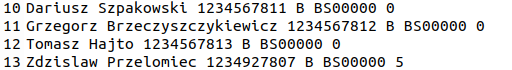
\includegraphics[width=0.75\textwidth] {customers}}
	\caption{Format danych w pliku Customers.txt:
	{\footnotesize \textit{IMIĘ...NAZWISKO...PESEL...KAT.PR.J....OBC.KONTA}}}
	\label{photo:customers}
\end{figure}

\begin{figure}[H]
	\centering
	\captionsetup{justification=centering}
	\frame {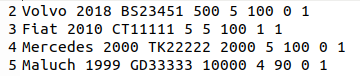
\includegraphics[width=0.75\textwidth] {cars}}
	\caption{Format danych w pliku Cars.txt:
	{\footnotesize \textit{NAZWA...ROK...NR.REJ...KOSZT...SIEDZ..SPRAW...CZYWYPOZ...CZYSPRAW}}}
	\label{photo:cars}
\end{figure}

\begin{figure}[H]
	\centering
	\captionsetup{justification=centering}
	\frame {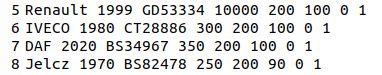
\includegraphics[width=0.75\textwidth] {trucks}}
	\caption{Format danych w pliku Trucks.txt:
	{\footnotesize \textit{NAZWA...ROK...NR.REJ...KOSZT...POJBAG...SPRAW...CZYWYP...CZYSPRAW}}}
	\label{photo:trucks}
\end{figure}
\subsection{Menu}
Menu zawiera mechanizmy zabezpieczające przed nieprawidłowymi danymi wejśćiowymi.
\subsection{Makefile}
Program można uruchomić z katalogu w terminalu przy użyciu \textit{make}:
\begin{itemize}
	\item \textit{make all} - tryb normalny (interaktywne menu)
	\item \textit{make test} - tryb testowy
	\item \textit{make clean} - usuwanie plików wykonywalnych
\end{itemize}

\section{Podział pracy}

\textbf{Michał Brus:}
\begin{itemize}
	\item Wstępne przygotowanie deklaracji klas i metod. 
	\item Metody VehicleRental: Add, Find, Delete, ShowOperationsHistory, Show...List, ShowInfo
	\item Klasa MyStack
	\item Main
	\item Makefile
\end{itemize}
\textbf{Łukasz Tumialis:}
\begin{itemize}
	\item Klasa Vehicle
	\item Testy
	\item Metody Load i Export oraz pliki z danymi 
	\item Metody VehicleRental: Rent, Payment, Return
\end{itemize} 
\textbf{Rafał Bednarz}
\begin{itemize}
	\item Klasa Customer
	\item Funkcje odpowiadające za IO
	\item Interaktywne menu
	\item Testy
\end{itemize}


\end{document}
